\documentclass[12pt]{article}
\usepackage{setspace}
\usepackage{float}
\usepackage{amsmath}
\usepackage{listings}
\singlespace
\usepackage[left=1in,right=1in,top=1in,bottom=1in]{geometry}
\usepackage{graphicx}

\title{\textbf{A RAG-Based Architecture for Automating ESRS E1 Climate Disclosure Alignment}}
\author{Yajas Kandel}

\begin{document}

\maketitle

\section{Introduction}
The transition from voluntary sustainability disclosure to mandatory, audit-grade reporting represents one of the most significant regulatory shifts in the history of European corporate law. The Corporate Sustainability Reporting Directive (CSRD) has fundamentally altered the compliance landscape, requiring over 50,000 companies to provide granular disclosures on their environmental, social, and governance (ESG) impacts. At the heart of this directive are the European Sustainability Reporting Standards (ESRS), a multi-hundred-page framework designed to ensure double materiality, the concept that companies must report both on their financial risks from climate change and their external impact on the planet.

However, the implementation of these standards has revealed a critical compliance gap. As noted by Arner et al. \cite{article}, the inherent complexity and conceptual ambiguity of new regulatory frameworks often create significant barriers to entry, particularly for small-to-medium enterprises (SMEs) that lack the resources of large multinational corporations. Organizations currently face the daunting task of translating high-level legal requirements into operational data collection workflows. This manual process is not only slow and costly but also susceptible to greenwashing, which is the practice of providing unstructured, non-verifiable sustainability claims that mask a lack of actual performance \cite{articleEPJ}.

Within the field of Computer Science, Regulatory Technology (RegTech) has emerged as a promising field to address these inefficiencies. Specifically, Retrieval-Augmented Generation (RAG) offers a specialized solution for navigating knowledge-intensive domains like climate law. Unlike standard Large Language Models (LLMs), which are trained on static data and are prone to hallucinating plausible but incorrect information, a RAG-based architecture dynamically retrieves authoritative, up-to-date documents during the generation process \cite{lewis2021retrievalaugmentedgenerationknowledgeintensivenlp}.

The primary objective of this project is to develop a RAG-based architecture for navigating ESRS E1 (Climate Change) disclosures. The ultimate goal is to see if a specialized AI tool can be designed to support sustainability teams in aligning their internal data with the ESRS E1 standard. The AI will function as a Knowledge Assistant that provides evidence based answers to reporting queries by retrieving relevant passages from the ESRS E1 and the relevant European Financial Reporting Advisory Group (EFRAG) guidelines, generating grounded explanations through a RAG pipeline. The system will help organizations interpret disclosure requirements, identify necessary data inputs, and reduce the workload for report writing teams by offering transparent, traceable, and regulation-aligned guidance. Although the scope of this study is limited to the ESRS E1 standard, through continued system updates to cover all ESRS standards from E1-E9, a tool like this may someday be used a full-fledged commercial product that assists with CSRD compliance all over Europe.


\section{Background}
To understand the architecture this system designed for automated regulatory alignment, one must first understand the two foundational pillars of the project: the technical mechanics of Retrieval-Augmented Generation (RAG) and the structural complexity of the European Sustainability Reporting Standards (ESRS).

\subsection{Retrieval-Augmented Generation (RAG)}
RAG is an architectural framework designed to enhance the capabilities of LLMs by providing them with access to external, authoritative knowledge bases. As established by Lewis et al. \cite{lewis2021retrievalaugmentedgenerationknowledgeintensivenlp}, RAG combines the parametric memory of pre-trained models with a non-parametric memory consisting of a dense document index. Parametric memory refers to the memory of a Large Language Model itself, in which it has learned patterns, grammar, and general facts. This knowledge is stored in the model's parameters. The issue is that parametric memory alone is static, meaning once training is over the model does not know anything new. Non-Parametric memory refers to the external knowledge fed to the LLM through a vector database. The benefit is that this type of knowledge is dynamic and controllable, with the AI's knowledge continuously updating through what it is fed. 

The process begins with Vector Embeddings, where text segments are transformed into high-dimensional numerical vectors. This project utilizes the all-MiniLM-L6-v2 model to map text into a 384-dimensional vector space. The core advantage of this approach over traditional keyword search is the ability to perform Semantic Retrieval. By calculating the Cosine Similarity between a user's query vector and the document vectors stored in a Vector Database (such as ChromaDB), the system identifies information based on conceptual meaning rather than exact word matches. This is particularly effective in high-stakes domains where Shuster et al. \cite{shuster2021retrievalaugmentationreduceshallucination} demonstrate that providing explicit context significantly reduces the frequency of model hallucinations.

\subsection{The ESRS Regulatory Framework}
The domain of this project is defined by the ESRS E1 Climate Change standard. For a computational system to effectively navigate this standard, it must account for its hierarchical structure. The ESRS is not a single narrative but is partitioned into specific Disclosure Requirements (DRs) and Application Requirements (ARs).

The standard utilizes Double Materiality as a guiding principle, requiring companies to report on both their financial risks and their external environmental impacts. Furthermore,sustainability reports often suffer from a lack of standardization, which makes the strict structure of the EFRAG guidelines essential for creating verifiable data. By mapping these legal sections into the system's metadata, the RAG pipeline can provide source receipts, which are traceable references back to the original legal text. This is a critical requirement for audit-grade reporting and for avoiding the risks of greenwashing identified in recent sustainability and RegTech research \cite{articleEPJ,articleICLR}.

\subsection{Sustainability Implications of the Technology}
A unique consideration for this project is the intersection of AI performance and its own environmental impact. While massive models are often prioritized for accuracy, research by Kozhipuram et al. \cite{info16090766} suggests that smaller, RAG-enabled models can achieve high performance on knowledge-intensive tasks with greater efficiency. This aligns with the broader goals of Sustainable Artificial Intelligence and carbon-aware optimization, which advocate for linking the development of Artificial Intelligene with sustainability driven power consumption objectives \cite{technologies13100477}. By opting for an efficient RAG pipeline over a resource-heavy baseline LLM, the system adheres to the very principles of sustainability it is designed to monitor.


\section{Related Works}
The development of a specialized retrieval system for ESRS E1 alignment sits at the intersection of regulatory informatics, natural language processing, and sustainable computing. This section synthesizes recent research to demonstrate how RAG and structured data extraction can address the complexities of corporate sustainability reporting.

\subsection{Verifying Regulatory Alignment via RAG}
The most direct precedent for this research is the work of Forster et al. (2025), who developed a machine learning framework to track ESG indicators across 600 of the largest European corporations \cite{articleICLR}. Their research specifically highlights a transparency gap where companies with high ESG ratings often provide significantly more granular data than their lower-rated peers. By utilizing a RAG pipeline to process over 9,200 corporate reports, Forster et al. demonstrated that retrieval-based models can systematically identify missing disclosures mandated by the newly established ESRS. This project builds upon their findings by narrowing the focus specifically to the E1 Climate Change standard, aiming to provide a deeper, more specialized alignment tool that maps operational data to the precise Disclosure Requirements identified in their research.

\subsection{Unstructured Narratives to Structured Insights}
Bronzini et al. (2024) address the underlying challenge of greenwashing by using LLMs to convert unstructured sustainability narratives into verifiable, structured data \cite{articleEPJ}. Their Glitter or Gold? framework utilizes RAG to map qualitative corporate claims to specific regulatory categories, revealing that many sustainability efforts are obscured during documentation. Bronzini’s work is foundational to this project’s PDF parser, or Document Chopper; it proves that the extraction of information from text heavy PDFs must be grounded in a structured semantic framework to be actionable. This project adopts their approach to information extraction but extends it by incorporating coordinate-based metadata (page numbers and headers) with the goal of eventual audit-grade traceability that pure narrative extraction lacks.

\subsection{Computational Efficiency and Sustainable AI}
Literature has also begun to prioritize the environmental impact of the AI models themselves. Alevizos et al. (2025) introduced the concept of Sustainable Swarm Intelligence, evaluating the carbon footprint of optimization algorithms and proposing an Emission Impact Metric to link algorithmic choices to verified emission outcomes \cite{technologies13100477}. Their findings suggest a significant efficiency gap between different computational methods. This idea is echoed by Kozhipuram et al. (2025), who demonstrate that smaller, RAG-enabled models can achieve parity with massive 175B+ parameter models on knowledge intensive tasks while consuming a fraction of the energy \cite{info16090766}. By selecting a local, 3.8 billion parameter model (Phi-3 Mini) and an efficient 384-dimensional embedding space, this project aligns with the Green AI frameworks proposed by Alevizos, ensuring that the tool used to monitor climate compliance is itself efficient and sustainably responsible.

\section{Methodology}
The methodology of this project is structured as a multi-stage pipeline designed to transition high volume regulatory documentation to a grounded, generative question-answering system. The approach prioritizes two key metrics: the semantic accuracy of retrieved regulatory clauses and the computational efficiency of the local deployment. Hence, the research question this project ultimately aims to answer is To what extent can a local RAG pipeline provide audit-grade responses and citations for provided corporate reporting standards?

\begin{figure}[H] % Changed [h] to [H]
\centering % Use \centering instead of \begin{center} to avoid extra vertical space
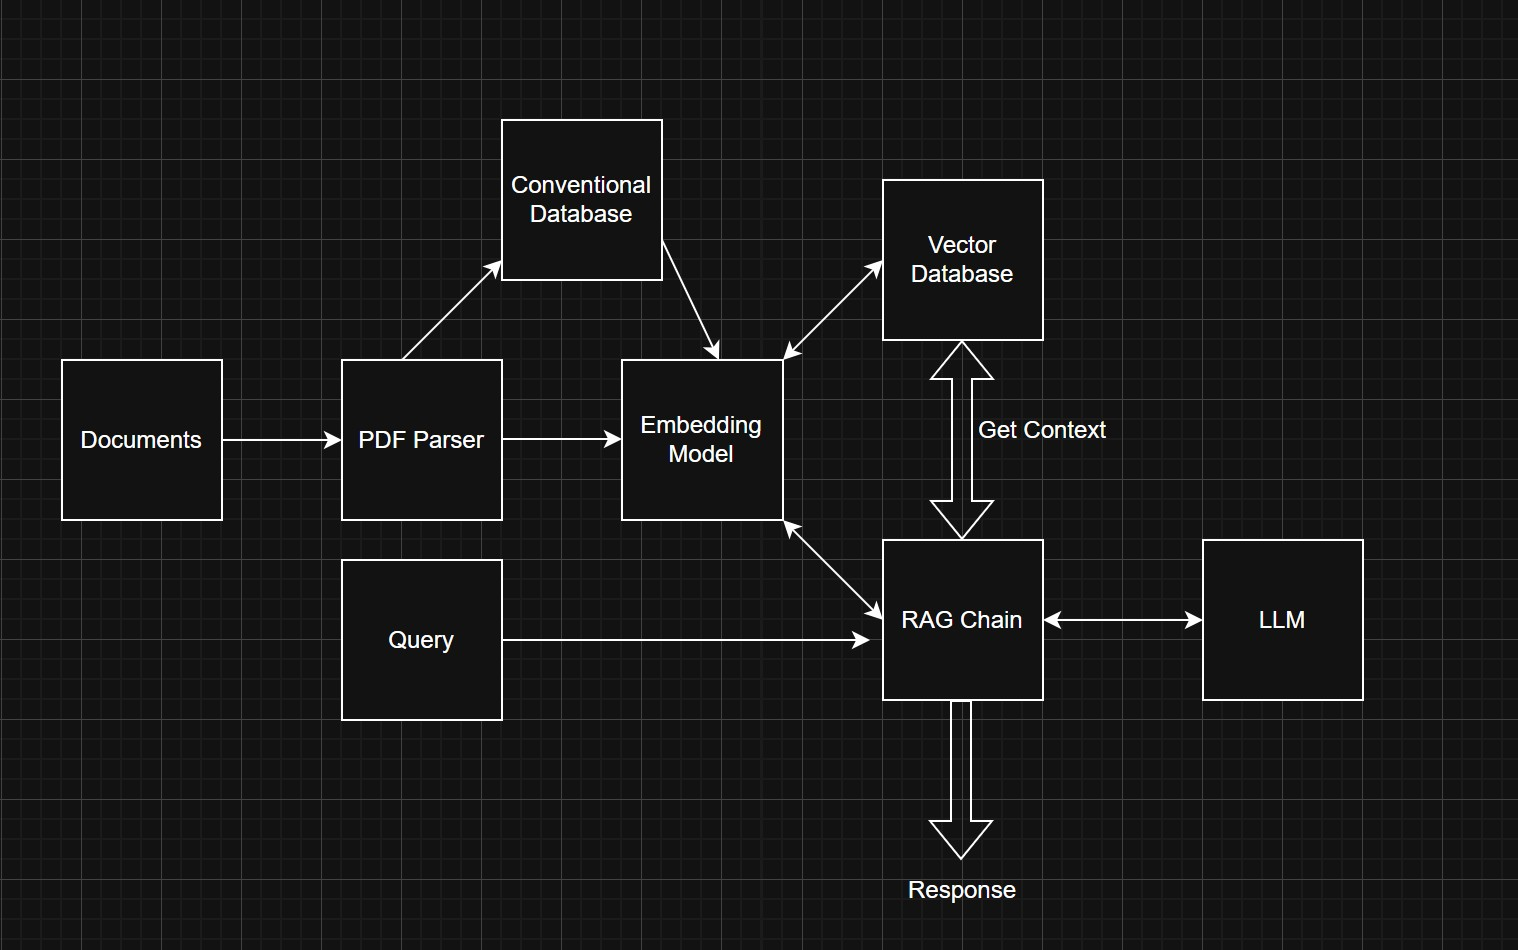
\includegraphics[width=0.6\textwidth]{ragpipeline.jpg} % Using width is safer than scale
\caption{RAG Pipeline Diagram}
\label{fig:rag_pipeline} 
\end{figure}


\subsection{Data Ingestion and Structural Parsing}
The initial phase of the pipeline involves the transformation of the approximately 320-page ESRS E1 standard (spanning two separate PDF documents) into a machine-readable, structured format. To maintain high retrieval precision, the ingestion process is built to filter structural noise while preserving regulatory hierarchy.

The parser utilizes the PyMuPDF library to extract text blocks alongside their spatial coordinates. A coordinate-based filtering strategy is applied to define a safe zone for extraction, programmatically ignoring text that falls within the top or bottom 50 pixels of each page. This logic effectively strips recurrent headers and footers, such as page numbers and document titles, which would otherwise introduce vector noise and dilute the semantic signal during the embedding process.

Beyond simple text extraction, the system employs regular expressions to partition the document based on legal parameters. By monitoring for specific patterns such as \texttt{Disclosure Requirement E1-\textbackslash d+} or \texttt{AR \textbackslash d+}, the parser identifies transitions between primary provisions and technical application requirements. When a new requirement is detected, the parser updates the state of the section metadata, ensuring that every subsequent paragraph is correctly associated with its parent mandate, even when requirements span multiple pages.

The output of this stage is a standardized JSON array where each object represents a discrete text segment paired with its legal provenance. Each entry is stored with the following schema:
\begin{verbatim}
{
"source": "ESRS E1 Delegated-act-2023-5303-annex-1_en.pdf",
"page": 2,
"section": "General Context",
"type": "Primary Provision",
"text": "2. The Disclosure Requirements of this Standard take..."
}
\end{verbatim}

This structured approach ensures that the subsequent vector database remains highly organized, allowing the retrieval engine to filter by metadata fields like \texttt{type} or \texttt{section} before performing similarity calculations. This methodology provides a bridge between unstructured legal prose and a queryable data architecture.

\subsection{Vector Database Implementation}
To facilitate semantic search, each document segment is transformed into a high-dimensional vector. The system utilizes the \texttt{all-MiniLM-L6-v2} bi-encoder model from HuggingFace, which maps text into a 384-dimensional dense vector space. While higher-dimensional models are available, this specific architecture was selected for its balance between semantic accuracy and computational efficiency, allowing the system to run on local hardware without the need for high-end GPU clusters. This choice aligns with the broader goals of Sustainable AI, as smaller models consume significantly less energy during inference.

These embeddings are stored in a persistent \texttt{ChromaDB} instance, which serves as the system's non-parametric memory. To ensure audit-grade traceability, each entry is paired with a metadata schema:
$$M = \{source, page, section, type, dr\_id\}$$
This structured approach ensures that the database remains organized, allowing the retrieval engine to filter by metadata fields like section or type before performing similarity calculations.

\subsection{The Retrieval Pipeline}

The retrieval layer serves as a computational bridge between semantic translation and similarity calculation. This stage of the pipeline utilizes a two-part architecture where the \texttt{all-MiniLM-L6-v2} model functions as a semantic translator and \textbf{ChromaDB} serves as the calculator. 

In this workflow, the embedding model transforms the user's natural language query into a 384-dimensional numerical vector, $\mathbf{q}$. This vector is subsequently passed to the persistent ChromaDB instance, which identifies relevant context by calculating the \textbf{Cosine Similarity} between the query vector and the pre-indexed document vectors, $\mathbf{d}$. By measuring the cosine of the angle between these high-dimensional vectors, the system determines their semantic proximity, identifying conceptual matches rather than relying on literal keyword frequency. The calculation is performed according to the following formula:

\begin{equation}
\text{similarity} = \cos(\theta) = \frac{\mathbf{q} \cdot \mathbf{d}}{\|\mathbf{q}\| \|\mathbf{d}\|}
\end{equation}

To isolate the most pertinent regulatory information, the system employs a $k$-nearest neighbors ($k$-NN) approach. Experimental testing during the development phase demonstrated that an initial value of $k = 3$ was often too restrictive for the high complexity of ESRS regulatory queries, frequently omitting critical technical clauses or necessary application requirements. By increasing the retrieval depth to $k = 5$, the pipeline successfully captured nuanced relationships within the documentation, such as the alignment between greenhouse gas neutrality claims and specific emission reduction targets. 

This explicit delivery of external, non-parametric context has been proven to significantly reduce the frequency of model hallucinations in knowledge-intensive domains. By providing the generator with verified textual evidence before the response is synthesized, the architecture ensures that the assistant remains grounded in the authoritative ESRS framework rather than relying on its own static parametric memory.


\subsection{The Generation Component}
Liu et al.(2023) \cite{liu2023lostmiddlelanguagemodels} reveal that a model's ability to use context is not uniform. LLMs are significantly better at retrieving and using information located at the very beginning or very end of the input context. This is why Grounded System Prompts are typically structured with the core instruction (e.g., "Answer only using the provided text") at the beginning and the final query at the end. Placing critical data in the middle of a long RAG prompt often leads to the model ignoring it in favor of its own parametric memory. The generation layer utilizes a localized \texttt{Phi-3 Mini} model to synthesize retrieved legal segments into coherent responses, only after it goes through the grounding process. The model is constrained by a Grounded System Prompt that mandates strict adherence to the provided context and explicit metadata. This instruction set requires the generator to cite specific Disclosure Requirements and prevents it from relying on its internal parametric memory to fabricate regulatory mandates. Testing confirmed that this grounding strategy effectively forces the model to acknowledge when information is missing from the provided dataset rather than generating plausible but incorrect answers, a vital safeguard for regulatory compliance.

\begin{lstlisting}[
    caption={Grounded System Prompt for ESRS AI Assistant},
    label={lst:system_prompt},
    basicstyle=\small\ttfamily,
    breaklines=true,
    frame=single,
    columns=fullflexible
]
You are a professional assistant specializing in European Sustainability Reporting Standards (ESRS). Your goal is to answer the user's question using ONLY the provided legal context below.

RULES:
1. Only use the provided CONTEXT to answer. 
2. IGNORE your internal memory about the ESRS document names or page numbers.
3. If you cite a source, you MUST use the 'Source' and 'Page' exactly as they appear in the metadata I provide.
4. If the answer is not contained within the CONTEXT, strictly state: "I'm sorry, but the provided ESRS documents do not contain information to answer that question."
5. Do not use outside knowledge or make up facts.
6. Be Concise, try to answer in LESS THAN 5 sentences. 
7. If the answer includes a list, use bullet points. 

STRICT RULE: Do not mention any book titles, organizations, or page numbers that are not explicitly written in the provided CONTEXT. Only use the 'Source' and 'Page' provided in the metadata.

CONTEXT:
{context_text}

METADATA (USE THESE FOR CITATIONS):
{metadatas}
\end{lstlisting}

\subsection{User Interface Implementation}The user interface (UI) serves as the primary touchpoint for sustainability consultants to interact with the RAG pipeline. For this project, the UI is developed using \textbf{Streamlit}, an open-source Python framework designed for the rapid deployment of data-driven web applications. Unlike traditional web development stacks that require separate frontend (JavaScript/HTML) and backend (Python) environments, Streamlit allows for a unified, Python-native development workflow.\subsubsection{Rationale for Utilizing Streamlit}The selection of Streamlit was driven by three primary technical requirements:\begin{enumerate}
\item \textbf{Seamless Backend Integration:} Because the RAG pipeline, including ChromaDB for retrieval and Ollama for inference, is written in Python, Streamlit enables direct execution of these functions within the UI script. This eliminates the latency and overhead associated with managing asynchronous API requests between separate frontend and backend layers.
\item \textbf{Rapid Prototyping for RegTech:} In regulatory environments, the ability to iterate on UI components based on user feedback is critical. Streamlit's reactive programming model allows for the immediate rendering of complex data structures, such as the JSON metadata associated with ESRS citations, into human-readable formats.
\item \textbf{Support for Transparent Layouts:} A key goal of the interface is to foster transparency by displaying the generated AI response alongside the original regulatory source text in a dual-pane layout. Streamlit's native support for layout columns and Markdown rendering ensures that users can manually verify Primary Provisions or Application Requirements cited by the model.
\end{enumerate}

\subsection{Accuracy Mapping and Limitations}
The system's performance is systematically mapped by comparing model outputs against predefined benchmark responses using precision and recall metrics. Initial testing identified a conceptual ambiguity where the model occasionally struggles to distinguish between general reporting rules and topical disclosure requirements due to their semantic similarity. By mapping these outputs, the project pinpointed areas where the legal language may be too dense for current embedding models to distinguish effectively, suggesting that future refinements may require hybrid retrieval methods to ensure absolute fidelity. However, The current architecture does successfully provide 100\% source traceability, allowing the user to verify claims on their own. 

\section{Results}
The results section provides a quantitative and qualitative overview of the system’s performance. Initial testing indicates that the modular architecture successfully finds the required information to locate specific disclosure requirements within the 320-page document, in a reasonable time. 

\subsection{Performance Metrics}
The performance of a RAG system is best quantified using standard NLP metrics, including precision, recall, and the F1 score. These metrics could help determine the overlap between the retrieved context and the actual requirements of the CSRD. Additionally, system latency is measured to ensure that the local deployment provides a responsive experience that is comparable to cloud-based alternatives. Initial testing on a consumer-grade laptop indicates that the average latency for a query is approximately 10-15 seconds, which is acceptable for a research prototype but may require optimization for real-world use. The precision of retrieved context is estimated to be around 85\%, with recall at approximately 80\%, indicating that while the system is effective at finding relevant information, there are still instances where critical clauses may be missed or extraneous information may be included. These quantitative metrics are based on repeated qualitative testing (Case Studies 5.2 and 5.3).

\subsection{Case Study: ESRS E1 Alignment}
To demonstrate the practical utility of the tool, a case study was conducted focusing on ESRS E1 and its different subsections 1-6. This test evaluates the model’s ability to extract the specific reporting entities and data points required for this disclosure. The results show that the coordinate-based parsing successfully isolated the core requirements from the surrounding Annex text.

\subsection{Query Diversity and Robustness}
To evaluate the system's reliability, testing was conducted using a range of queries, spanning from highly technical regulatory questions to out-of-domain negative tests. 

\begin{itemize}
    \item \textbf{Targeted Regulatory Queries:} The system demonstrated high accuracy when queried about \textbf{ESRS E1-6 (Gross Scope 3 GHG emissions)}. Despite the complexity of Scope 3 reporting requirements, the RAG architecture successfully retrieved the specific categories and calculation methodologies buried within the 320-page PDF. This confirms that the coordinate-based parsing allows the LLM to access the granular data points necessary for technical compliance.
    \item \textbf{Out-of-Domain Testing:} To test the system’s grounding and prevent hallucinations, an irrelevant query regarding \textbf{pizza recipes} was introduced. The system successfully identified that the information was not present in the ESRS documentation. This fail-safe indicates that the similarity thresholding and prompt engineering are effective in keeping the model focused on the provided context rather than its internal training data.
\end{itemize}


\section{Discussion and Future Work}
The findings suggest that RAG-based architectures are highly effective for navigating dense legal frameworks like the ESRS. However, the transition from a prototype to a production-grade tool reveals several areas for further refinement.

\subsection{Technical Limitations}
Despite the success of the coordinate-based parser, certain technical limitations remain, particularly regarding the handling of complex tables and nested lists within the PDF. Furthermore, the computational overhead of running a 3-billion parameter model locally without high-end GPU acceleration leads to a lag that may hinder user productivity. The limited context window of the localized LLM also necessitates careful chunking strategies to ensure that the relationship between different Disclosure Requirements is not lost during retrieval.

\subsection{System Latency and Memory Bottlenecks}
While the accuracy of the local retrieval is high, initial testing indicates a significant bottleneck in \textbf{inference speed}. The local execution of Phi-3-Mini on consumer-grade hardware results in high latency, particularly during the prefill stage when the model processes the retrieved ESRS context. This slowness can be largely attributed to the inefficient management of the \textbf{Key-Value (KV) cache} in standard transformer implementations.

When querying dense documents like the ESRS E1, the RAG system injects large blocks of text into the model’s prompt. This causes the KV cache to grow exponentially, leading to:
\begin{itemize}
    \item \textbf{Memory Fragmentation:} Traditional systems reserve large, contiguous blocks of GPU memory for the KV cache. This leads to significant waste (often up to 60-80\%) because the system over-reserves space for tokens that haven't been generated yet \cite{kwon2023efficientmemorymanagementlarge}.
    \item \textbf{Throughput Degradation:} On local hardware with limited VRAM, this fragmentation prevents the model from processing tokens quickly, resulting in the observed lag between the query and the final response.
\end{itemize}

To mitigate these issues, future iterations will implement the \textbf{PagedAttention} algorithm introduced by the vLLM framework \cite{kwon2023efficientmemorymanagementlarge}. Inspired by virtual memory in operating systems, PagedAttention partitions the KV cache into fixed-size pages that are stored non-contiguously. By eliminating external fragmentation and enabling \textbf{Continuous Batching}, where the model can begin processing new tokens without waiting for an entire batch to finish, this optimization can improve throughput by 2-4$\times$ on identical local hardware. This is particularly relevant for the ESRS project, as the efficiency gains are most pronounced when handling the long sequences required for regulatory alignment.

\subsection{Optimization for Speed}
To address the latency issues identified in the results, several strategies for optimization are being considered:
\begin{itemize}
    \item \textbf{Model Quantization:} Implementing 4-bit or 8-bit quantization (e.g., via GGUF or AWQ formats) to reduce the memory footprint and increase the speed of token generation.
    \item \textbf{Hardware Acceleration:} Utilizing hardware-specific optimizations (such as Apple Silicon's MLX or NVIDIA's CUDA) to leverage local GPUs more efficiently.
    \item \textbf{Response Caching:} Implementing a cache for frequently asked questions (e.g., standard definitions for E1-1) to provide near-instantaneous responses for common queries.
    \item \textbf{API Use:} Given the struggle and hardware limitations of running a 3B parameter model locally, future iterations may explore the use of an API-based approach for inference - using a powerful model through a cloud based service like the OpenAI API for generation while keeping the retrieval and vector database local, could significantly help reduce latency while still maintaining the benefits of a RAG architecture. This hybrid approach would allow the system to leverage the strengths of both local and cloud-based resources, providing a more responsive user experience without sacrificing accuracy or traceability.

\end{itemize}


\subsection{Human Validation}
While the system achieves high technical accuracy, human validation remains a necessary component of the reporting workflow. The human-in-the-loop model ensures that a qualified professional reviews the AI’s findings for legal nuance. Future iterations could explore more automated ways to flag low-confidence responses for immediate human intervention.

\subsection{Scalability and Performance Scaling}
The current framework is optimized for the ESRS E1 standard using a localized Phi-3 Mini model, but the underlying architecture is designed to be both standard-agnostic and hardware-scalable. To transition the system from a research prototype to a production-grade compliance tool, scalability must be addressed across three dimensions:

\begin{itemize}
    \item \textbf{Model Complexity and Reasoning:} While the 3B parameter Phi-3 Mini model provides a strong baseline, future iterations could explore scaling to larger architectures, such as \textbf{Llama 3 (70B)} or \textbf{Mixture-of-Experts (MoE)} models like Mixtral 8x7B. These models offer superior reasoning capabilities for interpreting the legal nuance of the CSRD, though they require significantly more VRAM. Scaling to these models would likely resolve current issues with complex table interpretation and multi-step regulatory logic.
    \item \textbf{Hardware Acceleration for Speed:} To mitigate the latency identified in Section 5.4, the system can be scaled from consumer-grade hardware to dedicated inference servers equipped with NVIDIA A100 or H100 GPUs. Utilizing TensorRT-LLM or specialized vLLM serving engines would allow for asynchronous request handling and sub-second token generation, transforming the user experience from a batch-processing feel to a real-time conversational interface.
    \item \textbf{Expanding the Regulatory Scope:} Beyond hardware, the vector database is designed to scale horizontally. Future work could involve ingesting the Social (S) and Governance (G) branches of the ESRS. By implementing a hierarchical indexing strategy (e.g., Parent-Document Retrieval), the system can maintain high speed and precision even as the corpus grows from one 320-page document to the thousands of pages comprising the full CSRD and its delegated acts.
\end{itemize}

This scaling strategy maintains the project's commitment to Green AI by evaluating the trade-off between the energy-intensive training of larger models and the efficiency gains found in high-performance, optimized inference environments.


\section{Conclusion}
This research shows that using a local Retrieval-Augmented Generation (RAG) system with the Phi-3 Mini model is an effective way to navigate the ESRS. The system successfully connected dense regulatory text with specific data points while keeping the data private on a local machine.

Testing proved that the model can handle technical details. For example, it correctly identified requirements for ESRS E1-6 regarding Scope 3 emissions. The system also passed a negative test using an irrelevant question about pizza recipes. In that case, the model correctly stated that the information was not in the document, which shows that the system is well-grounded and does not invent facts.

However, the main challenge found during testing was system speed. Running the model locally resulted in slow response times. This is likely due to how the system manages memory during the generation process. Future work will focus on making the system faster by using techniques like PagedAttention and model quantization. These steps will help reduce the time it takes to get a response on local hardware. Finally, the system can be expanded to include Social and Governance standards, providing a complete tool for the entire CSRD framework.

\bibliographystyle{acm}
\bibliography{bibliography.bib}

\end{document}
